%=========================================================================
% (c) 2011, 2012 Josef Lusticky

\chapter{Design}
For implementation of reasonably useful NTP client,
operating system must be able to set, get
and eventually adjust the system time in a similar fashion as
described in section~\ref{sec:system-keeping-and-providing} and~\ref{sec:system-discipline}.
Though not mandatory, adjusting time is important function,
if the time shall be always a monotonically increasing function.
Apart from that, communicating abilities over UDP are also required.

For developing and testing Contiki NTP client,
the AVR Raven platform with 8-bit ATmega1284P CPU~\cite{avr-datasheet} will be used.
This platform features IEEE~802.15.4 (Low-Rate Wireless Personal Area Networks) link layer support.
Together with an adaptation layer called 6LoWPAN (IPv6 over Low power Wireless Personal Area Networks)
AVR Raven is able to communicate over IPv6.

How to get a working setup with Contiki on this platform is described in
the document files on the CD enclosed to this thesis.
The CD content hierarchy is listed in appendix~\ref{app:cd-content}.

%... This is not in Contiki, as operating systems targeted at embbeded systems produce only 1 binary file. CITATION

%=========================================================================
% (c) 2011, 2012 Josef Lusticky

\section{Network communication}
Thanks to uIP, described in section~\ref{sec:contiki-uip},
the network communication is not a matter for Contiki OS.

intended to be used between different processes

AVR Raven features IEEE~802.15.4 (Low-Rate Wireless Personal Area Networks) link layer support.
On top of this layer, an adaptation layer called 6LoWPAN (IPv6 over Low power Wireless Personal Area Networks)
is used to communicate over IPv6 by Contiki.

Figure~\ref{fig:design-6lowpan} shows a complete hierarchy of network layers
concerned with NTP communication.
\begin{figure}
  \centering
  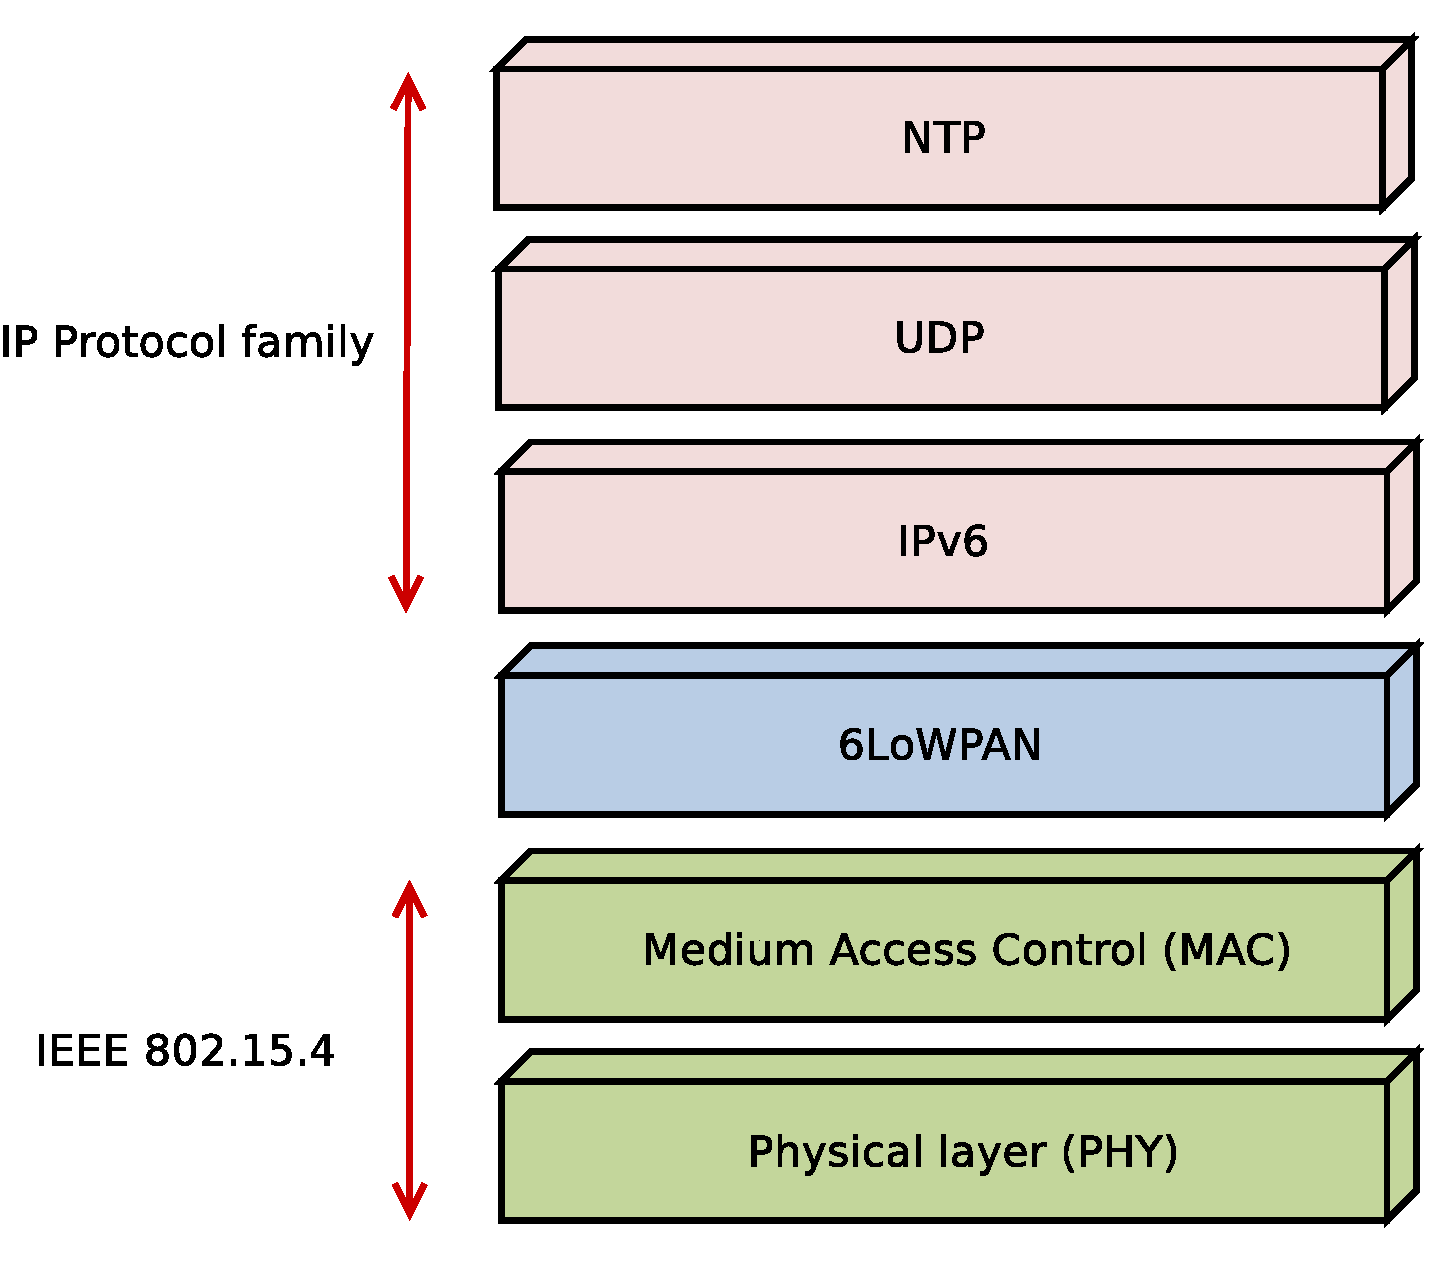
\includegraphics[width=9cm,keepaspectratio]{fig/6lowpan.pdf}
  \caption{Communication stack with 6lowpan layer}
  \label{fig:design-6lowpan}
  \bigskip
\end{figure}




%=========================================================================
% (c) 2011, 2012 Josef Lusticky

\section{Clock library extension}\label{sec:design-clock}
Previous section described how the call for getting the time acquires
the maximum precision the clock model allows.
Two read operations are needed in such a design - read {\it{scount}} and read {\it{TCNT2}}.
Since the {\it{scount}} variable depends on asynchronous interrupts produced by
the clock module, the followed query of the counter register causes a race condition.
The timer clock runs asynchronously from the CPU clock and
the result may be unpredictable if read while the timer is running.
Although the read could be wrapped with an interrupt disable,
the common solution on AVR platform in Contiki is to perform more read operations,
compare the results and perform read operations again if the results are not consistent.
Figure~\ref{fig:design-read} shows such a solution.

\begin{figure}
  \centering
  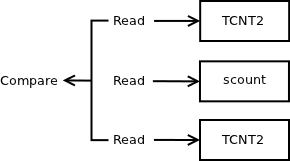
\includegraphics[width=6cm,keepaspectratio]{fig/read.png}
  \caption{Multiple read and result comparison}
  \label{fig:design-read}
\end{figure}

The call for adjusting the time computes the number of clock ticks
with the longer or shorter tick interval.
For storing the result, a new variable must be introduced.
If the value of this variable is zero, no adjustments are in progress.
Otherwise, the default value of the compare register is incremented or decremented by 1
and written to {\it{OCR2A}}.
This effectively causes adjusting the time, as described in section~\ref{sec:analysis-interface}.
When the time was adjusted enough,
the default value of the compare register is written back to {\it{OCR2A}}.

When adjusting the time in Contiki on AVR Raven, the as follows:
Section~\ref{sec:analysis-clock-interface} explained, that the default value
of the compare register for AVR Raven in Contiki is 31,
but the number of counter register increments between two successive interrupts is 32.
Incrementing the compare register value causes one real second to be experienced as
$\frac{f_{T2}}{CLOCK\_SECOND \times (32 + 1)} = \frac{4096}{128~\times~33} = 0.\overline{96}$~seconds
by the operating system.
Decrementing the compare register value causes one real second to be experienced as
$\frac{f_{T2}}{CLOCK\_SECOND \times (32 - 1)} = \frac{4096}{128~\times~31} \doteq 1.032258$~seconds
by the operating system.

Each increment of the counter register {\it{TCNT2}} takes
$\frac{1}{128 \times 32} = 0.000244140625$~seconds.
This is also the minimal possible clock adjustment,
that can be achieved by changing the compare register value just for one clock tick.
The fastest possible adjustment is approximately 0.03~$\frac{s}{s}$.
If faster adjustments were needed, the compare register would have to be updated with different values. 
However, updating the compare register with more different values would require
a more complicated software design
and lower values could cause a miss of the compare match described in section~\ref{sec:analysis-hwclock}.

% TO NTP INTERFACE
%When writing to compare register, the value is transferred to a
%temporary register, and latched after two positive edges of a source clock~\cite{avr-datasheet}.
%The user should not write a new value before the contents
%of the temporary register have been transferred to its destination.
%To detect that a transfer to the destination register has taken place,
%the Asynchronous Status Register - ASSR has been implemented.
%Since writing to compare register occurs only once within interrupt CONTEXT, % context?
%this detection is not mandatory.


%=========================================================================
% (c) 2011, 2012 Josef Lusticky

\section{Time interface extension}\label{sec:analysis-interface}
Section~\ref{sec:analysis-time} described, that there is no proper
way of setting, getting and adjusting the time for an NTP client in Contiki OS.
A new interface for setting, getting and eventually adjusting the time
must be therefore developed.

Setting the time should not cause a misbehaviour of the Contiki timers
described in section~\ref{sec:analysis-time}.
A modification of the {\it{scount}} and the {\it{seconds}} variable must be therefore avoided.
This can be achieved using an additional variable, containing the system boot time,
and modifying only that variable by the call for setting the time.
This way, the {\it{seconds}} variable will be further representing the system uptime
and the current real time can be obtained by $boottime + seconds$.
Since the {\it{scount}} also can not be changed, setting the time is only possible
within a precision of one second.
%Finer time setting must be made using the time adjustments.

By contrast, a call for getting the current time must be able to provide a higher precision.
Therefore, a new time specification structure must be designed as well.
To conform to the POSIX standard~\cite{posix}, this structure should consist of two parts -
one representing seconds and the other representing nanoseconds.
The first part represents the number of elapsed seconds since the POSIX epoch.
The nanosecond precision was chosen as modern systems also aim towards this
precision~\cite{posix,ntp-precision} and
the microsecond precision would also require at least 32-bit data type -
one second has 1~000~000 microseconds, which is more than the maximum expressible value of
an unsigned 16-bit data type $2^{16}$-1 (65~535).

The call for getting the time fills the time specification structure.
The part representing seconds is simply filled with the value of $boottime + seconds$,
while the part representing nanoseconds should be filled with the maximum precision
the clock model allows.
As described in section~\ref{sec:analysis-time},
this can be achieved by reading the {\it{scount}} variable
and by querying the hardware counter that is used for
interrupt generation and includes the time passed since
the last update of the {\it{scount}} variable.
This way, the resolution of
$\frac{1}{CLOCK\_SECOND~\times~counts} = \frac{1}{128~\times~32} = 0.000244140625$~seconds
can be acquired,
where $counts$ is the number of counter register increments between two successive interrupts,
which is 32 by default on AVR Raven, as stated in section~\ref{sec:analysis-clock-interface}.
%If this part was filled by only using the {\it{scount}} variable,
%just the resolution of the timer interrupt frequency would be provided.

Since setting the current time is possible only within one second precision,
finer time setting must be made using the time adjustments.
Section~\ref{sec:analysis-time} explained, that adjusting the time
should use the hardware clock as much as possible.
Adjusting the time changes the value in {\it{OCR2A}} compare register
to delay or shorten the clock tick interval,
which in turn speeds up or slows down the system time.
If the amount of required adjustments is positive, then the system clock is speeded up
until the adjustment has been completed.
If the amount of required adjustments is negative, then the clock is slowed down in a similar fashion.
Since the application specifies the amount of adjustments by the timestamp,
a new call must be developed for the determination of how many
clock ticks will be delayed or shortened, respectively.

As a result of this design, a leap second occurrence will be handled like an unexpected change of time -
the operating system will continue with the wrong system time for some time,
but an NTP client will set or adjust the system time~\cite{ntp-faq}.
This will effectively cause the leap second correction to be applied too late,
what is a trade-off for smaller memory requirements.


%%=========================================================================
% (c) 2011, 2012 Josef Lusticky

\section{Contiki NTP client}\label{sec:design-client}
The client application itself is a Contiki process,
which will use the designed operating system interface from the previous sections
and the uIP communication stack.

The client is able to use both NTP communication modes,
the NTP broadcast mode and the NTP unicast mode.
If the client will use only the broadcast mode, the structures and code
related to the unicast mode should not be included in the resulting program.
NTP broadcast mode packets can be received and processed from any NTP server in the network.
To avoid a complicated design when the NTP unicast mode is used,
the client is able to communicate only with one specified NTP server.

The NTP client fills and checks only the seconds part of the NTP timestamp,
because the conversion to the NTP format would increase the interval
between the timestamp determination and the dispatch of the filled packet.
After the filled NTP packet is sent, the client schedules
sending the next NTP packet in $2^{\tau}$ seconds %!LYDIA
by using the event timer library.
In NTPv4, $\tau$ ranges from 4, resulting in NTP poll interval of 16 seconds,
to 17, resulting in NTP poll interval of 36 hours.
However, the event timer library imposes a limit on the scheduled time.
This limit is platform specific and depends on the {\it{CLOCK\_SECOND}} value,
e.g. the $\tau$ value can not be greater than 8 on AVR Raven assuming 128 interrupts per second.
Upon scheduling the event timer, the client process yields
and another process could be run.
The client process is later invoked either by the uIP stack event
announcing the server response
or by the event timer in case no server response arrived.

Due to a missing simple solution for IPv4 communication over IEEE~802.15.4 link layer,
only IPv6 communication will be tested on the AVR Raven platform.
DNS resolution is not supported for this reason
and the remote server must be specified by address.

The packet loss problem was described in section~\ref{sec:analysis-application}.
However, a packet loss is not an issue if the client process uses the event timer library.
In the broadcast mode, a lost server packet causes no setting or adjusting the system time.
The client simply waits without disruption for the next NTP broadcast message.
If the client needs to figure out its local clock offset at the moment,
it can query the server by using the NTP unicast mode.
In the unicast mode, the client process is invoked in response to the expired event timer
and queries the server again.

When the server response arrives,
the destination timestamp determination is one of the first tasks the client does.
After that, the client makes packet sanity tests, including
checking whether the response is from a synchronised server.
In the unicast mode, the Originate Timestamp is compared with the stored sent timestamp. %!LYDIA
The received packet is considered bogus in case of a mismatch and further processing is stopped. %!LYDIA
Otherwise, the NTP timestamps are converted to the local timestamp format and
the local clock offset is computed as described in section~\ref{sec:ntp-algorithms}.
After the local clock offset is computed,
the stored transmitted timestamp is immediately set to zero
to protect against a replay of the last transmitted packet.
In the broadcast mode, the received packet is always considered correct
and the local clock offset is computed as the difference between the local stored timestamp
and the received Transmit Timestamp.
The local clock offset determined from the broadcast mode
is influenced by the network propagation delay and therefore less accurate.
The NTP client could exchange several packets with the server to calibrate the propagation delay.
But since local variables can not be reused in the Contiki process when the process yields,
this would cause either an extra memory overhead or a complicated client design.

Dynamic increasing or decreasing the client's Poll interval in response to
Kiss-o'-Death packets, described in section~\ref{sec:ntp-network}, would also
require a complicated design.
The client instead assumes, that an exhausted NTP server rather drops the incoming
client's query than sending a response with the KoD code.

Section~\ref{sec:design-interface} described that the client uses the POSIX timescale,
whereas NTP uses the NTP timescale.
Since both timescales reckon the time in seconds, %!LYDIA
the number of seconds between the NTP epoch and the POSIX epoch
can be simply subtracted from the seconds part of the NTP timestamp.
But the conversion from the fraction part of the long 64-bit NTP timestamp to nanoseconds,
used in the local timestamp structure,
is one of the most problematic tasks for memory constrained systems.
An accurate conversion requires either floating point operations or operations including 64-bit numbers~\cite{c99}.
The conversion is given by
$nsec = fractionl \times 10^9 \div 2^{32}$, where $nsec$ is the nanoseconds part of the local timestamp
and $fractionl$ is the fraction part of the long 64-bit NTP timestamp.

Because there is no native hardware support for floating point nor 64-bit arithmetic operations,
the compiler supplies these operations in form of library, called {\it{libgcc}} in case of the GCC compiler,
which causes a significantly bigger resulting binary file
(kilobytes in case of floating point operations and hundreds of bytes in case of 64-bit operations).
The greatest common divisor of $10^9$ and $2^{32}$ is $2^9$,
so in fact, a relatively simple multiplication of $fractionl$ by $\frac{5^9}{2^{23}}$ must be computed.
This could be computed on 32 bits using sequential
divisions by the power of 2 and multiplications by the power of 5.
In the standard C programming language, the bitwise right shift operator divides the unsigned data type by the power of 2
and the bitwise left shift operator multiplies the unsigned data type by the power of 2~\cite{c99}.
Therefore, the multiplication by 5 can be done using two left shifts and
adding the original value ($5x = 4x + x$).
The only constraint is that the overall coefficient of these operations must not be greater than 1,
that is, the value must be in the range from $0$ to $2^{32}-1$ in every step.
Otherwise, the value could overflow and the result would be incorrect.
Division can not cause such a situation but multiplication could.
The original value could be divided by a greater divisor,
but this would lead to a greater inaccuracy due to the lost of the least significant bits.
Because of this, multiplication done as soon as possible provides more accurate results.
The ideal conversion sequence is therefore given by formula~\ref{equ:conversion}.
\begin{equation}
\label{equ:conversion}
%\frac{10^9}{2^{32}} = \frac{2^9 \times 5^9}{2^9 \times 2^{23}} =
%\frac{5^9}{2^{23}} =
nsec = fractionl \times \frac{5}{2^3} \times \frac{5}{2^3} \times \frac{5}{2^3} \times \frac{5^2}{2^3} \times \frac{5}{2^3}  \times \frac{5}{2^3} \times \frac{5^2}{2^3} \times \frac{1}{2^2}
\end{equation}
It must be noted, that the above presented conversion is not exactly accurate,
because the least significant bits are lost by right shifts. %!LYDIA by
The accuracy can be determined by looping through all the possible values of $fractionl$ %!LYDIA by
and comparing the results with the reference algorithm that uses the floating point operations.
Such a measurement reports the maximum error of 5 nanoseconds,
which is totally adequate for most platforms without the floating point unit or
for platforms where 64-bit multiplication is expensive.
The implementation of the above as well as the program used for the
error measurement can be found on the CD attached to this thesis.
The table of CD contents is listed in appendix~\ref{app:cd-contents}.

After the timestamps were converted, the local clock offset is computed
as given in section~\ref{sec:ntp-algorithms}.
Depending on the absolute value of the local clock offset,
the system time is either set or adjusted using the {\it{clock\_set\_time}}
or {\it{clock\_adjust\_time}} call, respectively.
The clock is set if the time difference is equal or greater than
the offset threshold value.
The NTP specification suggests 0.125~seconds as the default~\cite{rfc5905}.
Because the designed call for setting the time, described in section~\ref{sec:design-interface},
can set the time only within a resolution of one second,
the threshold value must be at least one second.

